\section{Example of an application in social network analysis}
\label{sec:applications}

In this section, we demonstrate how maximum clique based algorithms can be used as  tools for  
detecting overlapping communities in social networks. 
%In particular, such algorithms have the unique ability to detect communities that are overlapping, i.e. they allow multiple communities to have common vertices, which most other algorithms do not.
Finding overlapping communities is a challenging problem \cite{Fortunato_2010}. 
Most community detection algorithms extract mutually independent communities 
in a given network and therefore are not suitable for detecting overlapping communities.
Yet, in many real-world networks, it is natural to find vertices (or members) that belong to more than 
one group (or community) at the same time.
%In social networks, for example, an individual may belong to different circles at the same time, one circle based on work colleagues, another on family relationships, and a third on sport associations, etc. 

Cliques are used as fundamental building blocks in a number of community detection algorithms which aim at extracting overlapping communities (ref???). One such algorithm, the Clique Percolation Method (CPM) (ref???) detects communities by merging overlapping sets of adjacent cliques. The first step in the algorithm is to identify all cliques of size $k$ in the given graph. This is typical done by detecting all maximal cliques in the graph. Then, a new graph is constructed such that each vertex represents one of these $k$-cliques. Two nodes in this new graph are considered to be connected if the $k$-cliques that represent them share $k$?1 members. The cliques of the connected components in the new graph are merged into communities. Since a vertex can occur in more than one $k$-cliques simultaneously, this results in an overlapping communities structure.

We devised an algorithm based on a similar idea as the CPM, but instead of using a enumerating all maximal cliques, we use our heuristic (Alg 2) as the core clique detection algorithm. We extended our heuristic such that it retains the largest clique containing each node. In order to leverage merging cliques, we also included an option to extract cliques other than the largest. We implemented this by introducing a parameter $c$, which essentially runs the heuristic $c$ additional times using a random choice of vertex at each step instead of picking the largest. In total, $(c+1) \times n$ cliques would be collected, $c \times n$ using random selection of vertices, and $1$ with the largest vertex at each step of the heuristic. We also modified the pruning steps by discarding cliques that cannot be more than size $k$, instead of the maximum clique size. Since we only look for cliques that overlap at least by $k$ nodes, we can safely prune these out. This is achieved by replacing all occurrences of $max$ in Algorithm 2???, and removing Lines (2 and 3???) as we now don't need to keep track of the maximum clique size. After extracting the cliques, we perform a standard component analysis, similar to the one described in (ref??? - supplementary info of Pallla paper) of the clique�clique overlap matrix to merge the cliques into communities.


We tested our algorithm on LFR benchmarks (http://sites.google.com/site/andrealancichinetti/files) proposed in [Lancichinetti et al. 2008] to evaluate the performance of our algorithm. These benchmarks introduce heterogeneity into degree and community size distributions of a network. These distributions are governed by power laws with exponents $\tau_1$ and $\tau_2$, respectively. It allows the generation of overlapping communities using the parameters, $O_n$, the fraction of overlapping nodes and $O_m$, the number of communities each overlapping node is assigned to. It also provides other parameters to control the network topology, such as the mixing parameter $\mu$, which is the expected fraction of links through which a node connects to other nodes in the same community, the average degree $K$, the maximum degree $K_{max}$, the maximum community size $C_{max}$, and the minimum community size $C_{min}$. We chose these parameters similar to those in [ref???]. We set the average degree $K$ to 10, which is of the same order as most large real-world social networks. The node degrees and community sizes are governed by power law distributions with exponents $\tau_1$ = 2 and $\tau_2$ = 1 respectively. We set the maximum degree $K_{max}$ to 50, and the minimum and maximum community sizes $C_{min}$ and $C_{max}$ to 20 and 50 respectively. We varied the parameters the mixing parameter $\mu$, the fraction of overlapping communities $On$, and number of community each overlapping node belongs to $O_m$ to generate the graphs. We chose to vary these as opposed to the others since these would have the most profound impact on the network topology for overlapping community detection. We tried two values at either extremes, for each of these parameters, hence resulting in eight graphs in total in our testbed. For $\mu$ we used 0.1 and 0.3, for $O_n$, we used 10$\%$ and 50$\%$, and for $O_m$, we used 2 and 8.

We evaluated the performance of our algorithm using the {\it Omega Index} [Collins and Dent 1988] which is a metric to compare how welll two sets of clusters or communities agree with each other. The omega index is the overlapping version of the Adjusted Rand Index (ARI) [Hubert and Arabie 1985], and it considers pairs of nodes belonging to the same number of clusters (possibly none) to compute the index.

We define the set of clusters found as a cover $C=\{c_1, c_2, ..., c_k\}$ [Lancichinetti et al. 2009], where $k$ is the number of clusters found.In the case of overlapping communities, a node may belong more than one cluster. Let $N1$ and $N2$ be the number of communities in covers $C1$ and $C2$, respectively, the omega index $\omega$ is defined as [Gregory 2011; Havemann et al. 2011]

\begin{equation}
\omega(C_1, C_2) = \frac{\omega_u(C_1, C_2) - \omega_e(C_1, C_2)}{1 - \omega_e(C_1, C_2)}
\label{eqn-omega}
\end{equation}

The unadjusted omega index $\omega_u$ is defined as

\begin{equation}
\omega_u(C_1, C_2) = \frac{1}{M} \sum\limits_{i=0}^{max(N_1,N_2)} \left\vert{s_i(C_1)\cap s_i(C_2)}\right\vert 
\end{equation}

where $M = n(n-1) /2$ represents the number of node pairs and $s_i(C)$ is the set of pairs that appear exactly $i$ times in a cover $C$. The expected omega index in the null model $\omega_e$ is given by

\begin{equation}
\omega_e(C_1, C_2) = \frac{1}{M^2} \sum\limits_{i=0}^{max(N_1,N_2)} \left\vert{s_i(C_1)}\right\vert \cdot \left\vert{s_i(C_2)}\right\vert 
\end{equation}

The subtraction of the expected value in Equation \ref{eqn-omega} takes into account agreements resulting from chance alone. The larger the omega index is, the better the matching is between two covers. A value of 1 indicates perfect matching. When there is no overlap, the omega index reduces to the ARI.

We test three versions of our algorithm using different values for the parameter $c$ = 0, 2 and 5. When C is set to zero, it basically uses only the largest cliques for each node. As we increase $c$, more and more cliques are considered towards merging and community detection. Other than computing the omega index w.r.t the ground truth, we also compare it with the results of CFinder \footnote{http://www.cfinder.org}, an implementation of CPM, whose time complexity is polynomial in many applications [Palla et al.2005].

\begin{table}[!hbt]

\footnotesize
\scriptsize
%\small
\centering
\caption{blah blah. C=num of communities, S=num. shared nodes, $\tau$=time in seconds}
\label{tab:applications}
%\begin{tabular}{l@{\hspace{6pt}}r@{\hspace{6pt}}|@{\hspace{6pt}}r@{\hspace{6pt}}r@{\hspace{6pt}}r@{\hspace{6pt}}r@{\hspace{6pt}}|@{\hspace{4pt}}r@{\hspace{4pt}}r@{\hspace{4pt}}r@{\hspace{4pt}}r@{\hspace{4pt}}|@{\hspace{6pt}}r@{\hspace{6pt}}r}

\begin{tabular}{@{\hspace{2pt}}c@{\hspace{4pt}}  c@{\hspace{4pt}}  c@{\hspace{2pt}}  c | @{\hspace{2pt}}c@{\hspace{2pt}} || c@{\hspace{2pt}}  c@{\hspace{2pt}}  c@{\hspace{4pt}}  c@{\hspace{3pt}} | c@{\hspace{3pt}}  c@{\hspace{3pt}}  c@{\hspace{3pt}}  c@{\hspace{3pt}} | c@{\hspace{3pt}}  c@{\hspace{3pt}}  c@{\hspace{3pt}}  c@{\hspace{3pt}} | c@{\hspace{3pt}}  c@{\hspace{3pt}}  c@{\hspace{3pt}}  c@{\hspace{3pt}} }
\toprule\toprule
	&  			& 			& 			&  			& 		&		&	CFinder	&			&		&		&	New(c=0)	&			&		&		&	New(c=2)	&			&		&		&	New(c=5)	&			\\
$n$	&	$\mu$	&	$O_m$	&	$O_n$	&	C(GT)	&	C	&	S	&	$\omega$	&	$\tau$	&	C	&	S	&	$\omega$	&	$\tau$	&	C	&	S	&	$\omega$	&	$\tau$	&	C	&	S	&	$\omega$	&	$\tau$	\\
\hline\hline
1000	&	0.1	&	2	&	10\%	&	34	&	37	&	55	&	0.842	&	0.913	&	60	&	64	&	0.758	&	0.031	&	49	&	76	&	0.825	&	0.255	&	40	&	59	&	0.840	&	0.912	\\
1000	&	0.1	&	2	&	50\%	&	44	&	62	&	153	&	0.402	&	0.855	&	87	&	116	&	0.280	&	0.016	&	83	&	158	&	0.363	&	0.089	&	68	&	158	&	0.395	&	0.254	\\
1000	&	0.1	&	8	&	10\%	&	51	&	58	&	30	&	-0.002	&	0.732	&	76	&	46	&	-0.002	&	0.025	&	65	&	39	&	-0.002	&	0.159	&	61	&	35	&	-0.002	&	0.550	\\
1000	&	0.1	&	8	&	50\%	&	130	&	74	&	68	&	0.030	&	0.358	&	74	&	56	&	0.020	&	0.005	&	79	&	66	&	0.028	&	0.016	&	79	&	72	&	0.030	&	0.042	\\
1000	&	0.3	&	2	&	10\%	&	35	&	50	&	53	&	0.612	&	0.592	&	69	&	67	&	0.461	&	0.013	&	64	&	73	&	0.577	&	0.090	&	55	&	60	&	0.605	&	0.321	\\
1000	&	0.3	&	2	&	50\%	&	44	&	60	&	95	&	0.193	&	0.434	&	92	&	93	&	0.109	&	0.006	&	85	&	102	&	0.152	&	0.024	&	77	&	106	&	0.169	&	0.068	\\
1000	&	0.3	&	8	&	10\%	&	48	&	64	&	35	&	0.304	&	0.472	&	79	&	59	&	0.239	&	0.011	&	74	&	55	&	0.293	&	0.064	&	69	&	46	&	0.301	&	0.205	\\
1000	&	0.3	&	8	&	50\%	&	142	&	57	&	43	&	0.019	&	0.326	&	58	&	46	&	0.013	&	0.005	&	61	&	49	&	0.017	&	0.011	&	59	&	45	&	0.018	&	0.034	\\
\bottomrule\bottomrule
\end{tabular}

\end{table}



% (ref to supplementary info???).  


We developed a very simple clique-based community detection algorithm using our heuristic as follows. We modified our heuristic such that it retains the largest clique containing each node. We use the heuristic instead of the exact algorithm because it is much faster and delivers near-optimal solution which is sufficient for the purpose of detecting communities. It is possible that we get duplicate cliques via different nodes,  
and so we remove these. The resulting cliques are cohesively connected subgroups, and those are
what our algorithm outputs as communities.

%This is done by simply substituting Lines 3 and 4 of Algorithm \ref{alg:clqHeu}, with a simple routine that stores each clique in a preferred data structure. 


%A detailed overview of community detection methods, and the significance and complexity involved in overlapping community findingcan be found in \cite{Fortunato_2010}.


%\footnotetext{http://www.facebook.com}

For experiments, we generated a user-interest-based network using data collected from 
two widely used social media platforms: Facebook and Twitter.
%\footnote[1]{http://www.facebook.com}  and Twitter \footnote[2]{http://www.twitter.com}. 
Facebook {\it walls} and Twitter {\it profiles} are features in these platforms that provide a medium for businesses, groups and individuals to post content such as messages, promotions or campaigns. These features also engage other users by allowing them to reply or comment on the already posted content. We use users' comments on posts added on the Facebook {\it walls} as an indicator of their interests in the respective 
{\it walls}, and use this to formulate the network for our experiments. The user comments and user information from specific {\it walls} are publicly available and collected using Facebook API\footnote[3]{http://developers.facebook.com/}. Similarly, for Twitter, we deduce users' interests by using their {\it tweets}. 
A {\it tweet} is a message with up to 140 characters related to a particular Twitter {\it profile}. We use two kinds of {\it tweets}: {\it retweet}, which is a {\it tweet} made by a Twitter {\it profile} that gets tweeted again by another interested user, and {\it mentioned tweet}, which is a {\it tweet} made by an interested user regarding the Twitter profile. The publicly available user mentioned tweets, retweets of a Twitter profile, and information of users who tweeted on these profiles are collected using Twitter API\footnote[4]{https://dev.twitter.com/docs/}.



With the collected data, we use the following technique to generate our user-interest-based network. From the gathered Facebook data, we calculate, for each {\it wall} $i$, the total number of unique users $u_i$ who have commented on it, and for each pair of {\it walls} $i, j$, the number of common users who have commented on both {\it walls} $c_{ij}$. The same procedure is carried out for Twitter {\it profiles}. We then construct an undirected graph $G = (V,E)$, where $V$ represents the {\it walls} or {\it profiles} and $E$ represents edges between them. We assign an edge between a pair of vertices, if there is at least one common user between them. The edge weight $w_{ij}$, which indicates the strength of the connection, is computed using the 
Jacard index or similarity coefficient \cite{Leydesdorff} given by
%\begin{equation}
\[w_{ij} = \frac{c_{ij}}{u_i+u_j-c_{ij}}\]
%\end{equation}

It is clear from the above equation that the weight is between 0 and 1, a value closer to 1 implying the {\it walls}/{\it profiles} being more similar in terms of user interests.
We then convert the graph to an unweighted graph by pruning edges whose weights are below a specified threshold, thus retaining only the links that indicate strong correlation. The choice of the threshold is subjective, and determines the size, number and quality of communities detected by our algorithm. 

The weighted graph we formed using the Facebook data had 1144 vertices and 348,274, and that the Twitter graph had 1144 vertices and 204,131 edges. Since we look for the most cohesive subgroups, we set the threshold to a high number, that gave us fairly small communities with up to $\sim$15 vertices.


%For our small experiment, we use data collected from Facebook\footnote[1]{http://www.facebook.com}. Every user on Facebook has a {\it wall}, which is a the user's profile space that allows the posting of messages, often short or temporal notes by other users. The user comments and user information from specific {\it walls} are publicly available and we collected them using Facebook API. We constructed a graph with the {\it walls} as vertices. Any two users who have commented on the same {\it wall} indicate a connection between the {\it walls}, and we form an edge between them. There could be many common users for each wall, and so we assigned edge weights by Jacard index or similarity coefficient \cite{Leydesdorff}. Once this is done for all {\it walls}, we retained only those edges which have weights above a chosen threshold, indicating a strong correlation. The threshold is a user's choice and decides both the size and the number of communities found.
% If an edge already exists, we increase the edge weight by 1. Once this is done for all {\it walls}, the edge weights are normalized, and we retain only those edges which have edge weights above a chosen threshold (we use 0.01), indicating a strong correlation.

%duplicate removal
%We modified our heuristic to retain the largest maximum clique containing each node. 
%This is done by simply substituting Lines 3 and 4 of Algorithm \ref{alg:clqHeu}, with a simple routine that stores each clique in a preferred data structure. 
%The exact algorithm could have also been used instead of the heuristic for this purpose. We choose the heuristic since it is much faster and for this particular problem of community detection the accuracy of the size of cliques formed is not critical.


\begin{figure}%[h!]
  \centering
    %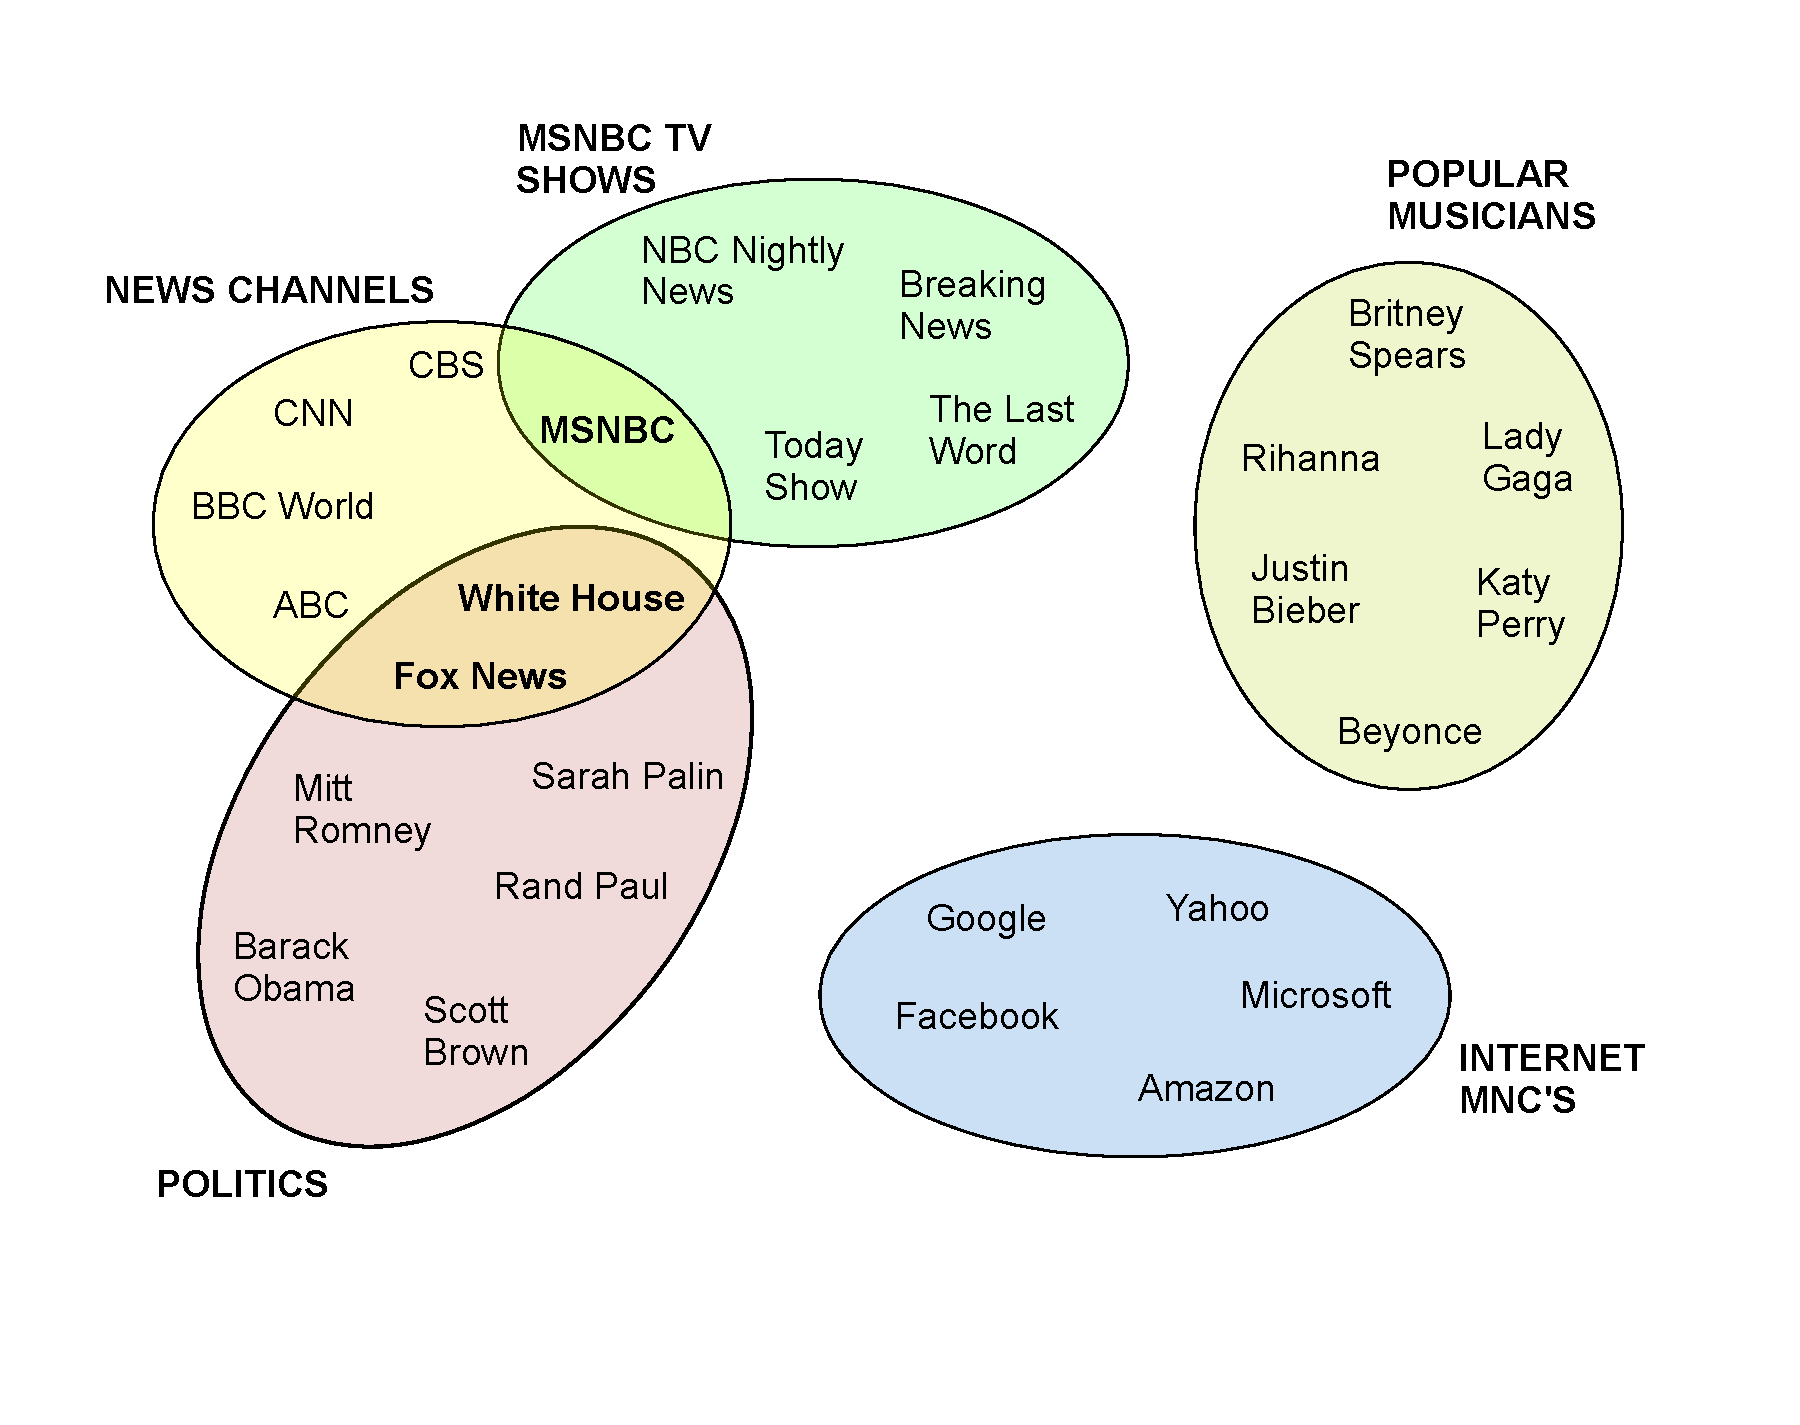
\includegraphics[width=1\textwidth]{communities_fb.pdf}
    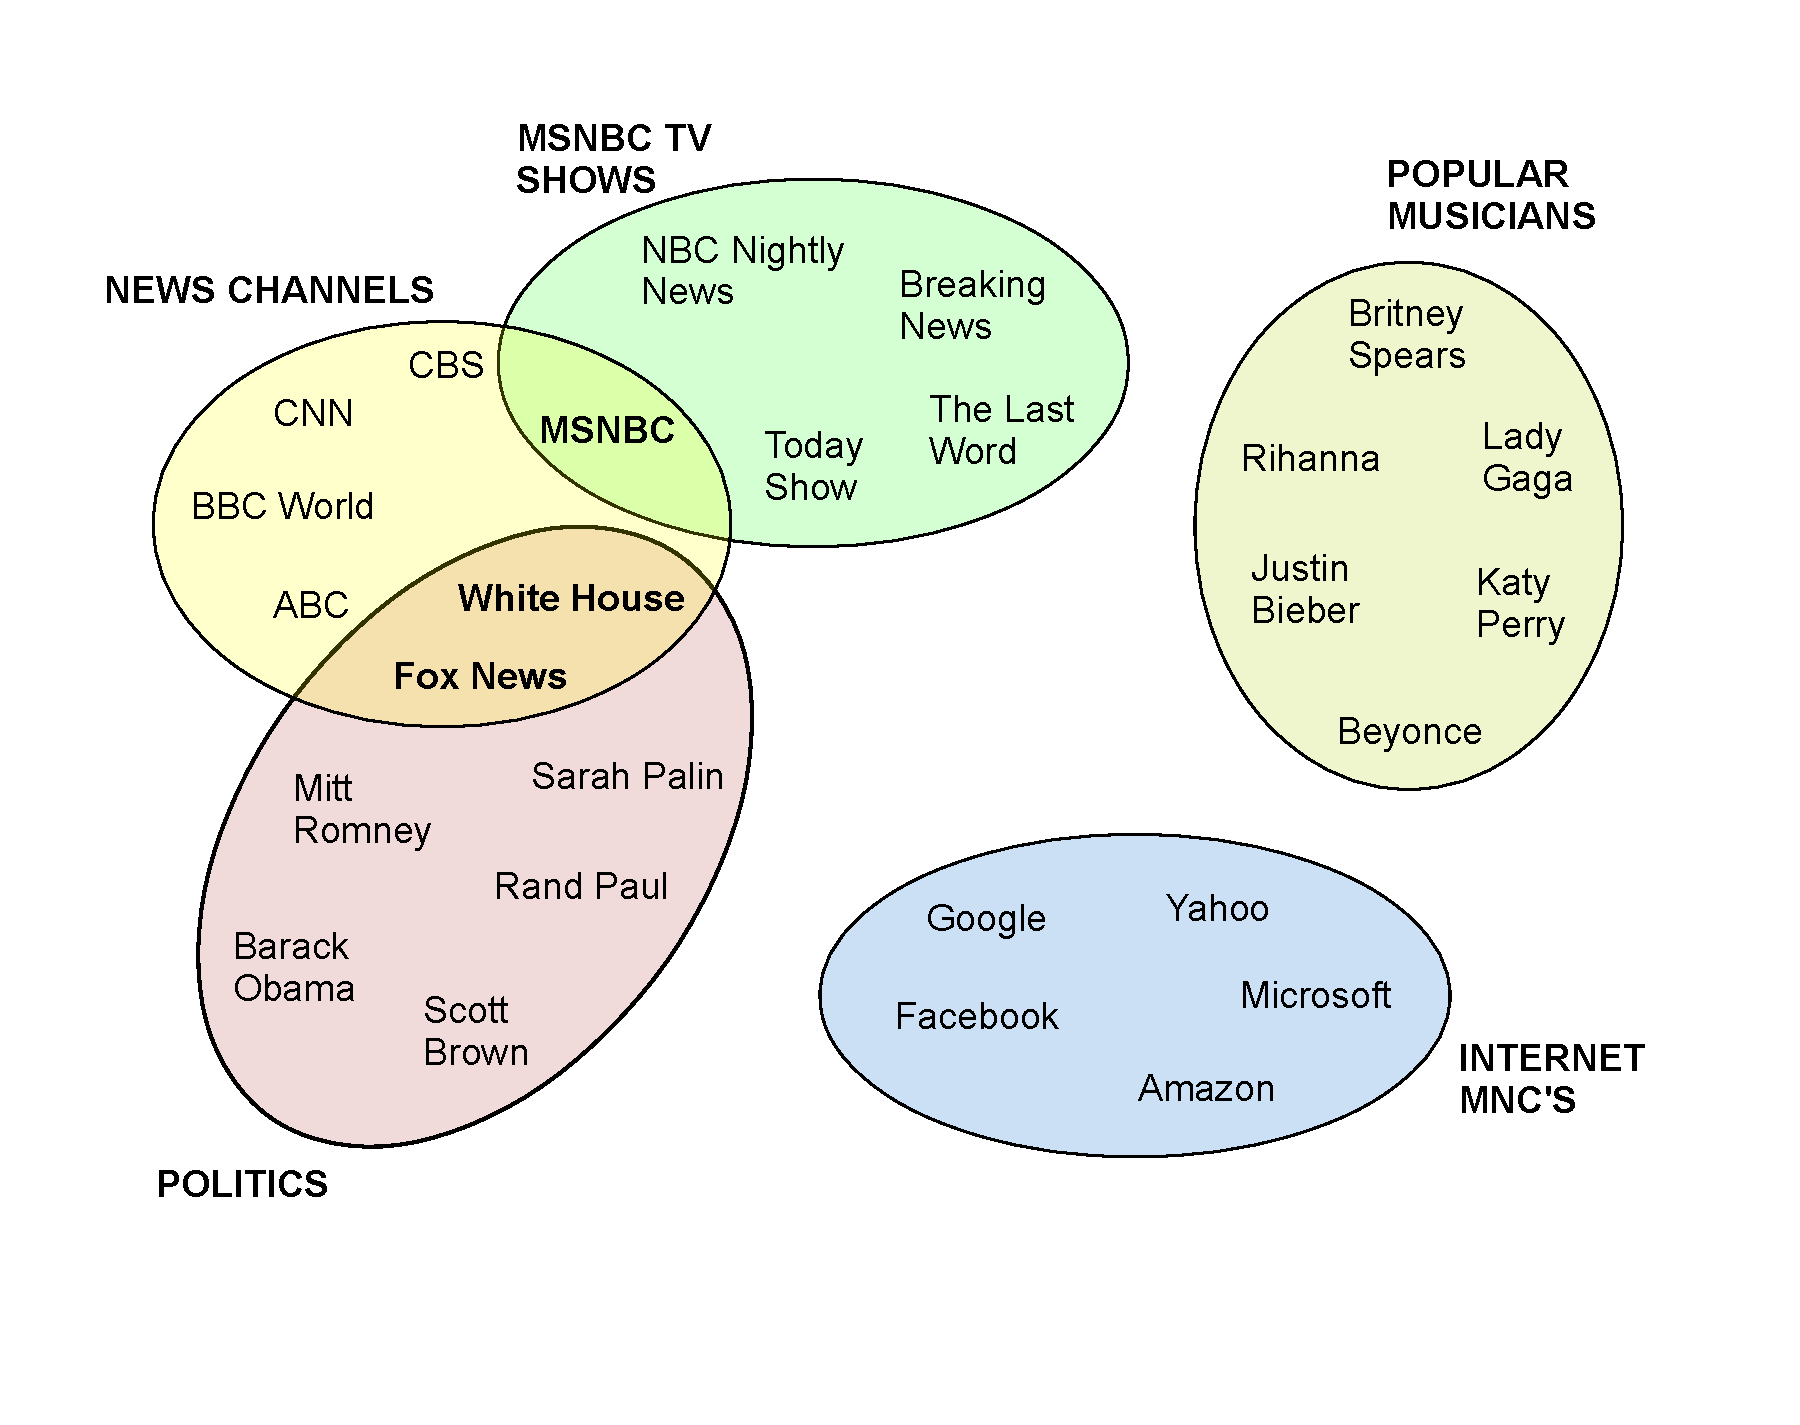
\includegraphics[scale=0.25]{communities_fb.pdf}
    
%\vspace{-30pt}
  \caption{Some Facebook communities detected by our algorithm.}
\label{fig-communities-fb}
\end{figure}
%\vspace{-10pt}

Figure \ref{fig-communities-fb} shows a few of the cliques/communities detected by our algorithm from the Facebook graph. A few cautionary points need to be pointed out here. The figure represents only a small subset of the communities detected by our algorithm, which we decided to present here to illustrate the results of our algorithm. In reality, a large number of communities ($\sim$100) similar to the ones shown here were detected. Furthermore, the members in the communities also represent only a subset of nodes that belonged to that community, and we decided not to show the rest to favor clarity and simplicity. In order to improve readability, we have also decrypted the names of the nodes, which in reality were Facebook or Twitter handles of {\it walls} or {\it profiles}. The original handles lacked spaces in between words, had special characters such as underscore, or had additional terms, all of which we decided to leave out to help the reader better comprehend the names.

As shown in Figure \ref{fig-communities-fb}, we obtained a number of isolated communities similar to the one of {\it popular singers}, and that of {\it internet corporations}. We also see communities that pertain to {\it MSNBC and its (news related) shows}, {\it news channels}, and {\it politics}. The point of this experiment is that our algorithm allows a node to be a member of more than one community and therefore helps detect overlapping communities. For instance, although the {\it news channels} and {\it MSNBC shows} communities are essentially separate, they share a common member, {\it MSNBC}, which is relevant to both. 
A similar feature can be observed between the {\it news channels} and  {\it politics} communities
where the two communities share two members. 
Figure \ref{fig-communities-tw} shows the communities detected from the Twitter graph. 
One can observe a very similar pattern there as well.
%add from nature paper why this is significant. coexistence of their structural subunits 

%\vspace{-20pt}
\begin{figure}%[h!]
  \centering
    %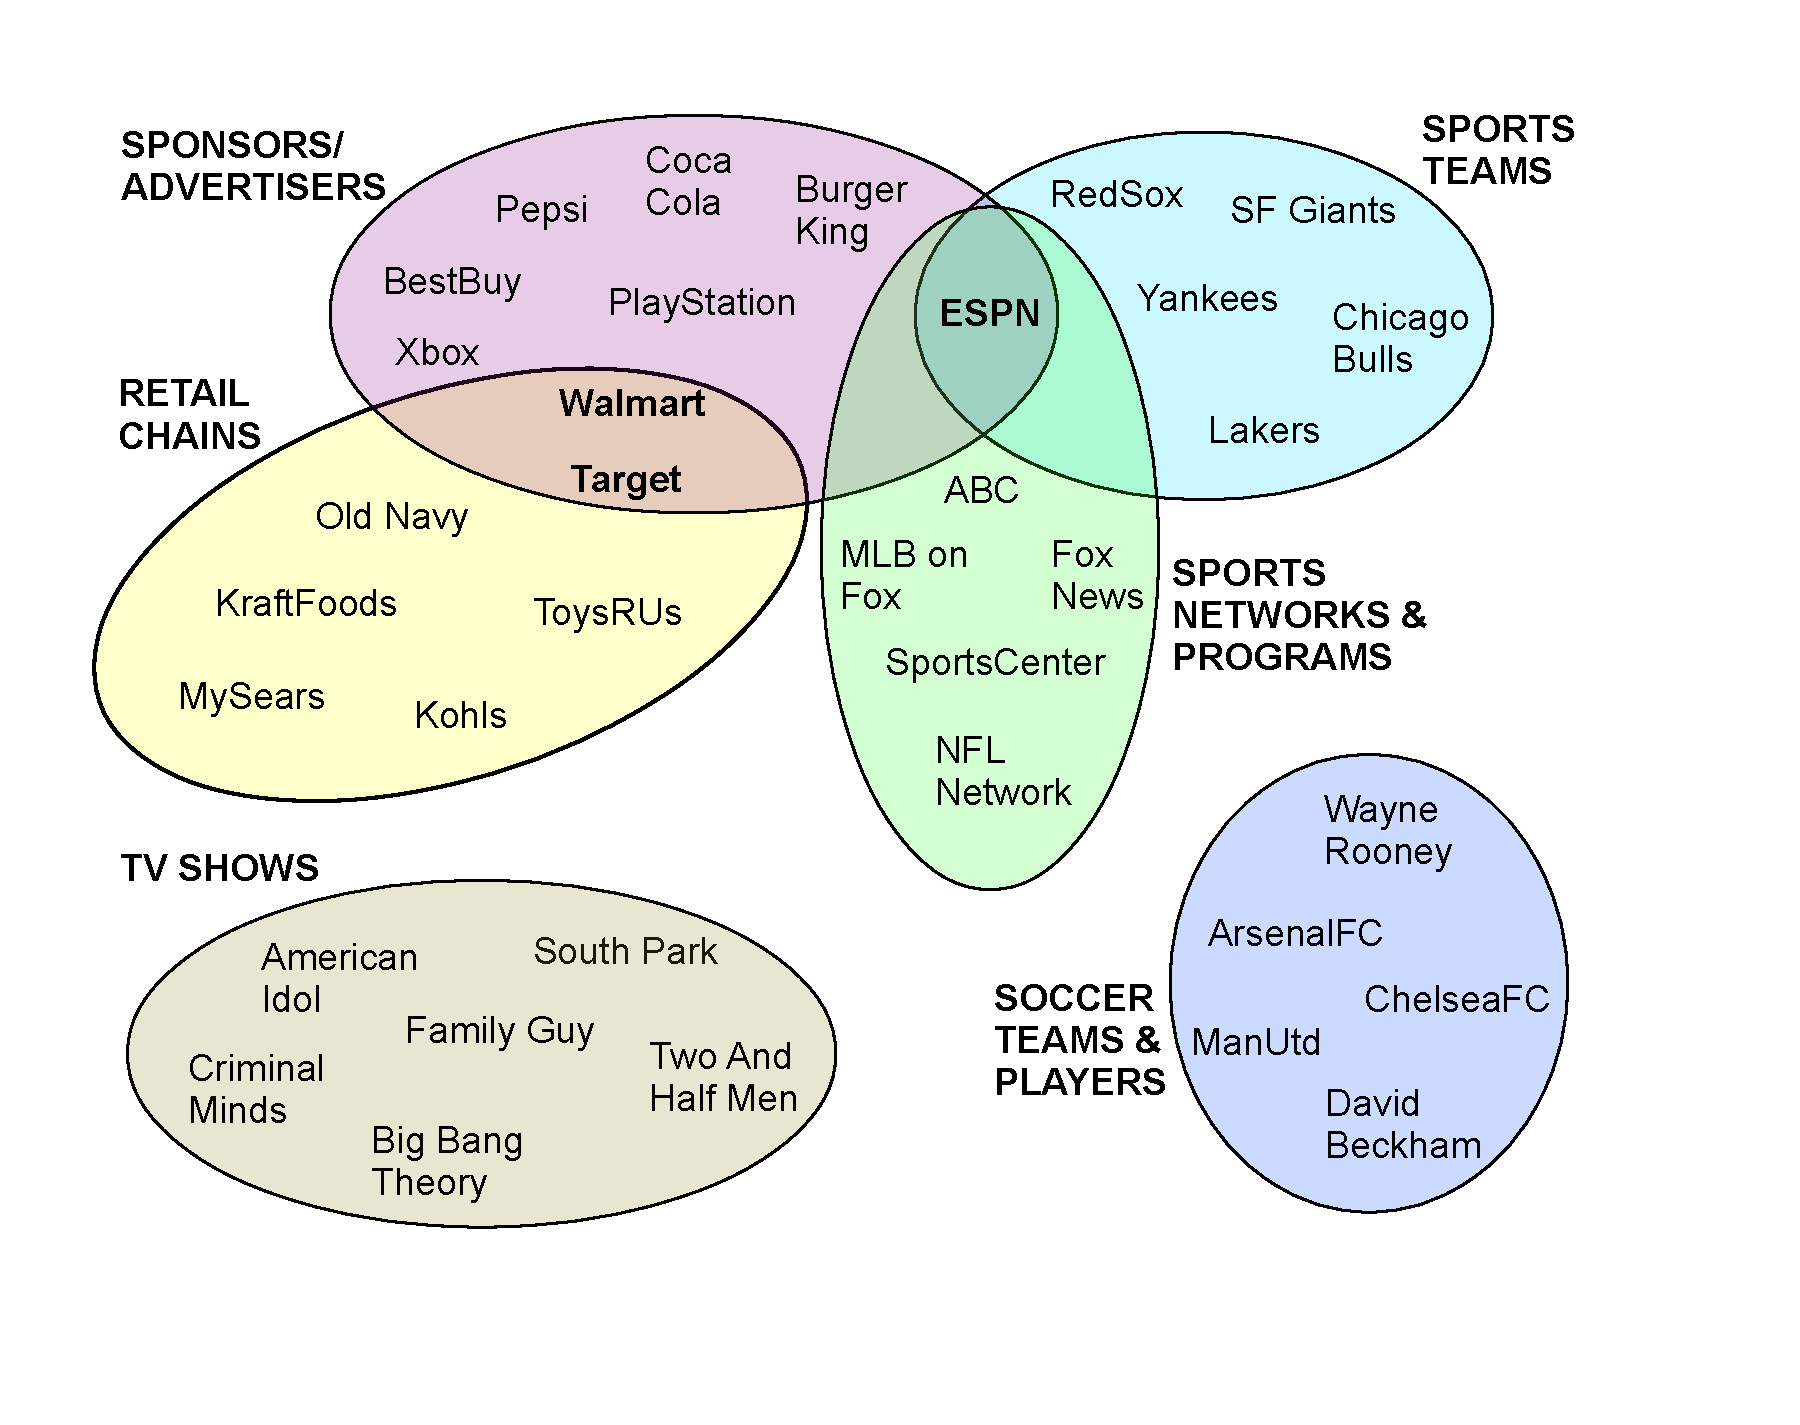
\includegraphics[width=1\textwidth]{communities_tw.pdf}
    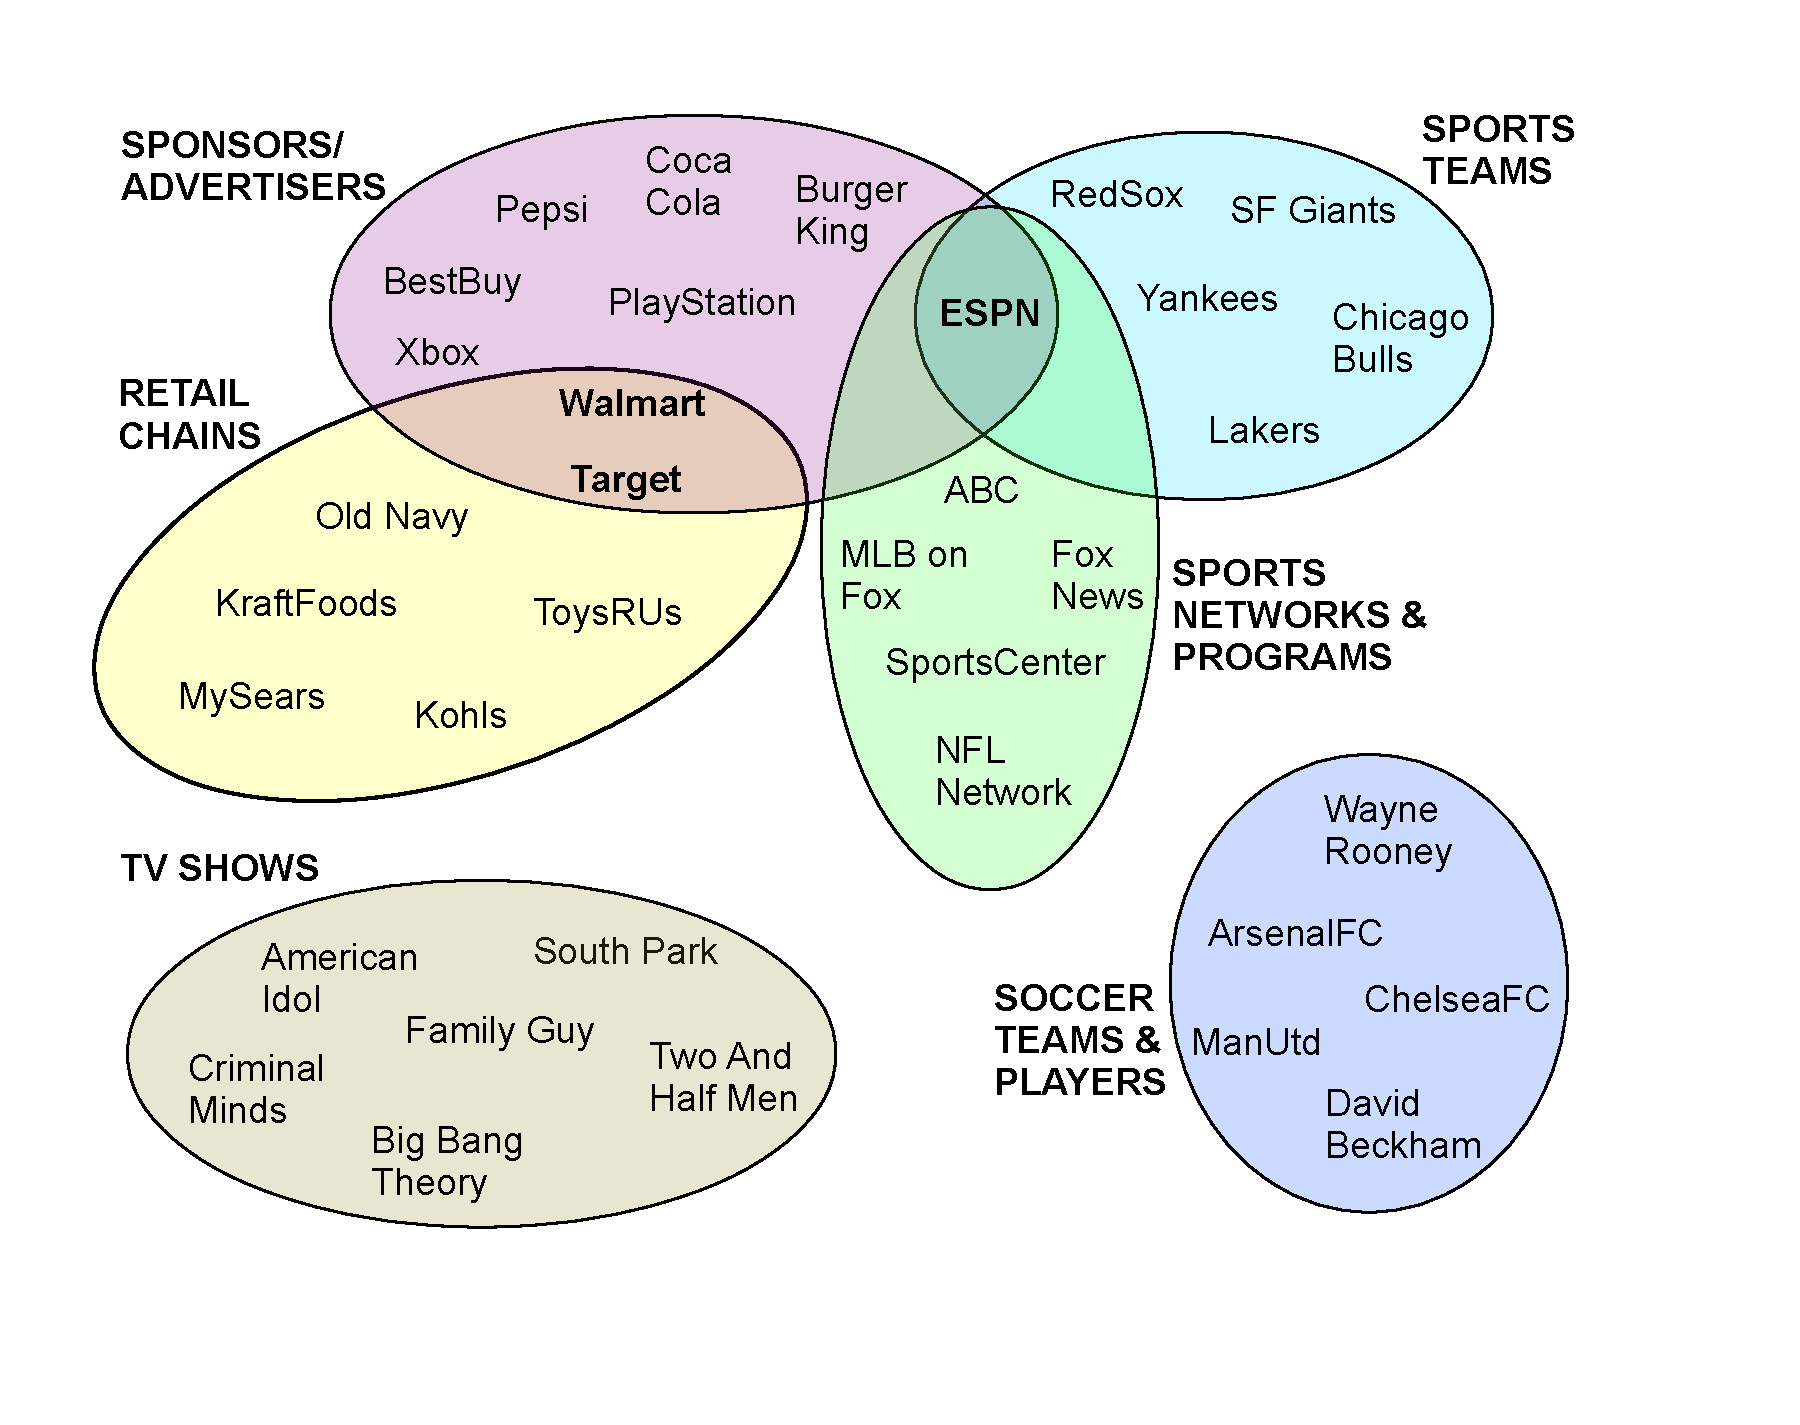
\includegraphics[scale=0.25]{communities_tw.pdf}
%\vspace{-30pt}
  \caption{Some Twitter communities detected by our algorithm.}
\label{fig-communities-tw}
\end{figure}
%\vspace{-10pt}


As demonstrated by these experiments, the algorithm used here although rather elementary can be effective at detecting overlapping communities. Our algorithm, however, detects communities formed by cliques, which is a stringent requirement. Appropriate relaxations, such as the use of $k$-cores, is worth investigating and is one of
the future lines of work we intend to pursue. 




%The immediate next thing to try would be to extend this to allow for clique-relaxations, such as $k$-core, $k$-plex \ref{Doreian1994267} etc. This can be done by merging the communities detected by our algorithm, which is one of the future lines of work we intend to pursue.
